\subsection{Testing for Browser cache weakness - OTG-AUTHN-006}
\subsubsection{BANK-APP}
\begin{longtable}[l]{ p{2.3cm} | p{.79\linewidth} }\hline
    & \textbf{BANK-APP} \\ \hline
    \textbf{Observation} &
        \begin{itemize}
            \item It is found that sensitive data is not saved anywhere throughout the application. This is achieved with the header \code{Cache-Control: must-revalidate, pre-check=0, post-check=0, no-store, no-cache}.
            \item The Back button of the browser neither re-logs the user in nor shows the last opened view.
         \end{itemize}
    \\
    \textbf{Discovery} &
            This vulnerability was detected using the Burp Suite, About Cache feature of the Firefox browser and manual testing. Steps are as follows:
                   \begin{itemize}
                      \item \textbf{Detecting cache headers - } The response headers were observed through the Burp Suite tool.

                      \begin{itemize}
                          \item In the browser, under Tools - set the Foxy Proxy Standard to use Burp Suite for all URLs. Open the Burp Suite tool.

                          \item  Open the site in the browser and login with credentials. Observe the response headers in Burp Suite to consist of the cache header as stated above. See Figure \ref{fig:burp_cache_header}

                          \item  Browser Cache was further inspected with Mozilla's built in tool (about:cache).
                      \end{itemize}
                      \end{itemize}
                      \\ &
                      \begin{itemize}
                      \item \textbf{Testing cache weakness -}
                        \begin{itemize}
                            \item Open the application in the browser and login with valid credentials.

                            \item The Transactions page is displayed. Click on the logout button.

                            \item User is redirected to the Login page. Click on the Back button of the browser.There is no redirection to the Transactions page, because of the Cache Control header that states that the cache should be revalidated. Hence user remains on the login page.
                      \end{itemize}
                   \end{itemize}
              \\
    \textbf{Likelihood} & Likelihood of the vulnerability is low since the attacker needs to change Cache Control header of the application, which requires technical knowledge about analyzing requests and how to modify them.\\
    \textbf{Impact} & N/A \\
    \textbf{Recommen\-dations} & N/A \\ \hline
    \textbf{CVSS} & N/A
    \\ \hline
\end{longtable}

\begin{figure}[ht]
	\centering
		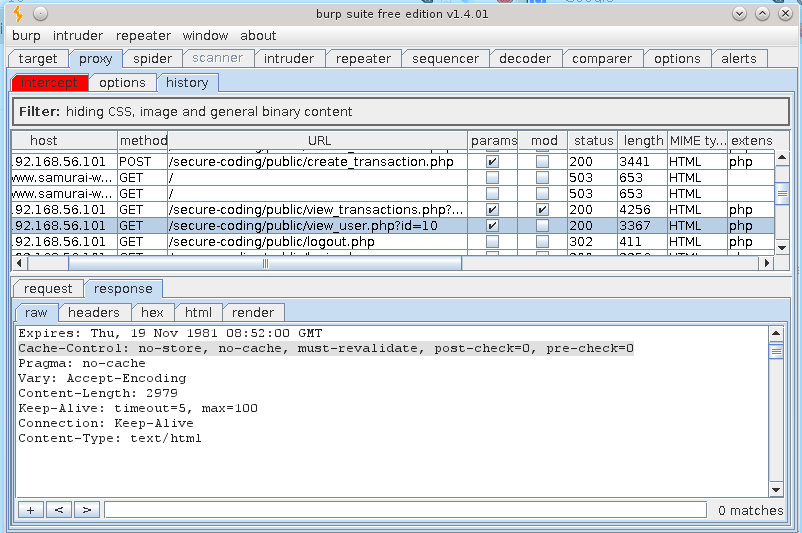
\includegraphics[width=.8\linewidth]{figures/OTG-AUTHN-006.png}
		\caption{BURP - Checking for cache headers}
	\label{fig:burp_cache_header}
\end{figure}

\subsubsection{SecureBank}
\begin{longtable}[l]{ p{2.3cm} | p{.79\linewidth} }\hline
    & \textbf{SecureBank} \\ \hline
    \textbf{Observation} &
        \begin{itemize}
            \item It is found that sensitive data is not saved anywhere throughout the application. This is achieved with the header \code{Cache-Control: must-revalidate, pre-check=0, post-check=0, no-store, no-cache}.
            \item The Back button of the browser neither re-logs the user in nor shows the last opened view.
        \end{itemize} \\
    \textbf{Discovery} & Same as described for BANK-APP. \\
    \textbf{Likelihood} & Same as described for BANK-APP. \\
    \textbf{Impact} & N/A \\
    \textbf{Recommen\-dations} & N/A \\ \hline
    \textbf{CVSS} & N/A
    \\ \hline
\end{longtable}

\subsubsection{Comparison}
Both of the applications behave similarly in this case and are secure since no sensitive data is stored in browser cache.
\clearpage